\documentclass[twoside,a4paper]{electhesis} %, nonatbib origtoc

\usepackage[parsec]{electhesis-tweaks}
\raggedbottom	% Dont stretch text in a page if it does not fit.

\usepackage{tabularx}							% A table package.

%%%%%  MATH, UNITS, SYMBOLS  %%%%%
\usepackage[tbtags]{mathtools}                  % Use amsmath + fixes
\usepackage{amsthm}
\usepackage{newtxmath}
\usepackage{bm}
\usepackage{nicefrac}
\usepackage[separate-uncertainty=true]{siunitx}                    % Correctly formatted units


%%%% Fixing the size of headings %%%%%
\renewcommand{\HeadFont}{\footnotesize}

%%%% Creating book-style headers. The ELECTHESIS's style can get messy at times. %%%
\usepackage{fancyhdr}
\pagestyle{fancy}
\fancyhf{}
\renewcommand{\chaptermark}[1]{\markboth{\MakeUppercase{\thechapter.\ #1}}{}}
\renewcommand{\sectionmark}[1]{\markright{\MakeUppercase{\thesection\ #1}}{}}
\fancyhead[LE, RO]{\PageFont\thepage}
\fancyhead[RE]{\HeadFont\leftmark}
\fancyhead[LO]{\HeadFont\rightmark}
\renewcommand{\headrulewidth}{1pt}
\renewcommand{\footrulewidth}{0pt}


\usepackage{appendix}	% Appendix package to handle appendices.

%% Change referencing symbols. %%
\usepackage[sort]{natbib}
\bibpunct{[}{]}{,}{a}{}{, }

%%%% Make sure day does not appear on the first page of title. %%%%
\usepackage[nodayofweek]{datetime}
\newdateformat{monthyeardate}{\monthname[\THEMONTH] \THEYEAR}


%%%%%  DOCUMENT METADATA  %%%%%
\phdthesis
%\methesis


%%%%%%%%%%%%%%%%%% Thesis title. %%%%%%%%%%%%%%%%%%%%%%
\title{\texorpdfstring%
	{This is the title of my thesis.} % Main title.
	{This is a shorter version of my title.} % Short title.
} % Usually the main and the short titles are same.

%%%%%%%%%%%%%%%%% Thesis author %%%%%%%%%%%%%%%%%%%%%%%
\author{John Doe}

%%%%%%%%%%%%%%%%% Time of thesis, current time by default. %%%%%%%%%%%%%%%
\date{\monthyeardate\today}

%%%%%  FONTS  %%%%%
\usepackage[T1]{fontenc}
\usepackage[utf8]{inputenc}


%%%%% Inline enumitem
\usepackage{blindtext}
\usepackage[inline]{enumitem}

%% I use oxford comma. if you don't, change {, and } to { and }
\sisetup{range-units=single,per-mode=symbol,list-units=single,list-final-separator={, and },detect-weight, detect-shape} 

\renewrobustcmd{\bfseries}{\fontseries{b}\selectfont}

%%%%%  Glossaries  %%%%%
\usepackage[xindy,style=super,shortcuts=abbr,abbreviations,nonumberlist,nomain,nogroupskip,automake,docdef=restricted]{glossaries-extra}
\setabbreviationstyle[abbreviations]{long-short-desc}
\glssetcategoryattribute{abbreviation}{glossdesc}{firstuc}
\makeglossaries

%%%%%  FIGURES  %%%%%
\usepackage{graphicx}                   % Include images
\usepackage[export]{adjustbox}
\usepackage{pdfpages}                   % Include PDFs
\usepackage{flafter}                    % Place floats after definition
\usepackage{subcaption}                 % Support for subfigures
\usepackage{lpic}                       % Labels over pictures
\usepackage{tikz-timing}                % Timing diagrams
\usepackage{tikz-3dplot}                % Simple 3D figures
\usepackage[mode=buildnew]{standalone}                 % Create figures in external tex files
\usepackage{rotfloat}

%%%%%  TABLES  %%%%%
\usepackage{booktabs}                   % Good-looking tables
\usepackage{multirow}                   % Span table rows
\usepackage{longtable}                  % Required for acronym list

%%%%%  SOURCE CODE  %%%%%
\usepackage{listings}                   % Format source code

%%%%%  PSEUDO CODE  %%%%%
\usepackage[chapter]{algorithm}         % Floating algorithm environment
\usepackage[noend]{algpseudocode}              % Format pseudo-code

%%%%%  FOOTNOTES  %%%%%
\usepackage{fnpct}                      % Kerning for footnotes near punctuation
\usepackage[bottom,perpage]{footmisc}           % Place footnotes below bottom floats
\usepackage{fnbreak}                    % Warn if footnotes break between pages

%%%%%  LINKS & REFERENCES  %%%%%
\usepackage[nohints]{minitoc}           % Insert in-chapter TOCs
\usepackage{nameref}                    % Reference the text of section headings
\usepackage[capitalize,noabbrev]{cleveref} % Automatic text in cross-references
\newcommand{\crefrangeconjunction}{--}

%%%%%  CONFIGURATION  %%%%%

\usepackage{xparse}                     % Define more powerful commands

\renewcommand\phi\varphi                % Prefer the variant phi glyph
\renewcommand\epsilon\varepsilon        % Prefer the variant epsilon glyph

\crefname{page}{p.}{pp.}                % Set page reference format
\Crefname{page}{Page}{Pages}

\usepackage{tabu}

% convert eps to pdf on the fly.
\usepackage{epstopdf}

% Path to figures.
\graphicspath{{figures/}}

% Rotating objects.
\usepackage{rotating}

\lefthyphenmin=4

%%%%% TikZ plots
\usepackage{tikz}
\usepackage{pgfplots}
\usepackage{grffile}
\usepackage{pgfplotstable}
\usepgfplotslibrary{patchplots,fillbetween,colorbrewer,groupplots}
\usetikzlibrary{calc,trees,positioning,arrows,chains,shapes.geometric,%
	decorations.pathreplacing,decorations.pathmorphing,shapes,%
	matrix,shapes.symbols,bayesnet,arrows.meta,plotmarks,patterns}

% Set your default pgfplot and tikz options, if needed.
\pgfplotsset{compat=newest}


% To have tables with footnote of the table.
\usepackage{threeparttable}

% Allow equations to spread in two pages.
\allowdisplaybreaks[1]

\begin{document}
	% Dont change these.
\renewcommand{\glossxtrsetpopts}{\glsxtrsetpopts{noindex=false}}
\newcommand*{\ifnotused}[3]{\ifglsused{#3}{#2}{\glsunset{#3}#1}}


%% Add your abbreviations.
%% \newabbreviation{key}{Short name}{Long name}
\newabbreviation{erp}{ERP}{event-related potential}
\newabbreviation{emg}{EMG}{electromyogram}
\newabbreviation{eog}{EOG}{electrooculogram}
\newabbreviation{eeg}{EEG}{electroencephalogram}

	% Stretch vertical space of tables.
	\renewcommand{\arraystretch}{1.1}

	\frontmatter
	
	% Create title page
	\maketitle

	% Create abstract page
	\unnumberedchapter{Abstract}

This is an example of abstract for thesis. You can use abbreviations such as {`\textbackslash ab\{eeg\}'} resulting in \ab{eeg}  or {`\textbackslash Ab\{eog\}'}, i.e., \Ab{eog}, to use capital for the starting letter. Using them again {`\textbackslash ab\{eeg\}'} will result in \ab{eeg} short version only.



	% Create Acknowledgements
	\unnumberedchapter{Acknowledgements}
\label{chap:Acknowledgements}

First and foremost, I would like to express my sincere gratitude to Prof. Richard Jones. 


	% Create table of contents page
	\cleardoublepage
	
	\addcontentsline{toc}{chapter}{{\textbf{CONTENTS}}}
	\tableofcontents

	% Create Acknowledgements
	\unnumberedchapter{Preface}

This thesis is submitted for the degree of Doctor of Philosophy in Electrical and Computer Engineering at the University of Canterbury. 


	%\renewcommand*{\glsgroupskip}{\vspace{-0.2cm}}
\renewcommand{\glsnamefont}[1]{\textbf{#1}}
%\glssetcategoryattribute{general}{glossdescfont}{small}

\printabbreviations[title={ABBREVIATIONS}]


	\mainmatter



% Actual thesis
\glsresetall

\chapter{Introduction}\label{chap:Introduction}

\section{Overview}\label{intro:overview}
This is an overview of what you see.

\subsection{New subsection}
You can create subsections, subsubsection, and so on.

Lets see an enumerate environment:
\begin{enumerate}
	\item this is an enumerate environment.
	\item You can just create items.
\end{enumerate}

Lets see an itemize environment:
\begin{itemize}
	\item this is an itemize environment.
	\item you can create bullet points.
\end{itemize}


\noindent There are times that you do not want to start a line with indentation. You can use `\textbackslash noindent' to make sure \LaTeX\ does not enforce it.
\section{Literature review} \label{chap:lit_review}

Here we want to refer to a previous chapter. For example, introduction chapter can be referred to as \cref{chap:Introduction}. `\textbackslash cref' can be used to refer to tables, figures, chapters, sections, and any other labels.
\chapter{Aim} \label{chap:aim}
\chapter{Methods} \label{chap:methods}

\cref{fig:1020EEG} shows a figure that we used with a caption. \cref{tab:interest} shows a table.


\begin{figure}[!htb]
	\centering
	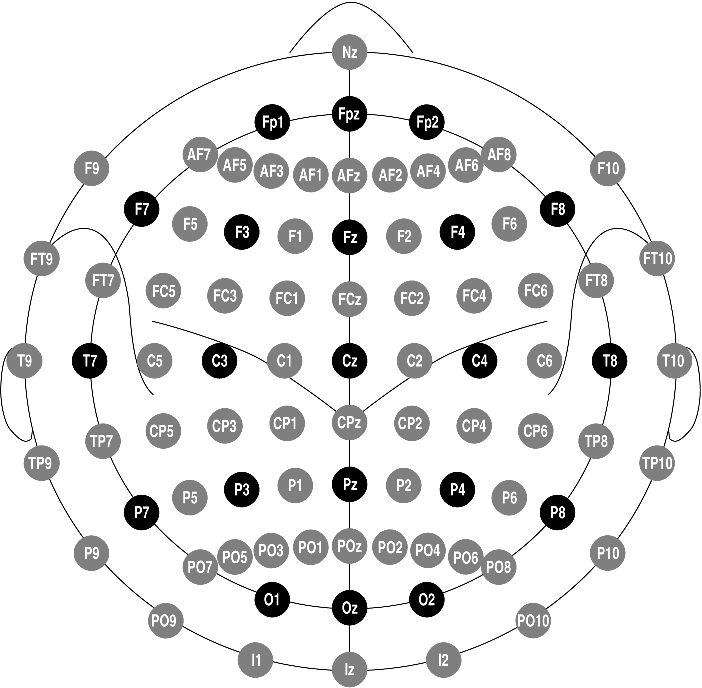
\includegraphics[width=2in]{figures/EEG_final_1020.pdf}
	\caption{An example of adding figures.}
	\label{fig:1020EEG}
\end{figure}

\begin{table}[!htb]
	\caption{A table of interest.}
	\label{tab:interest}
	\centering
	\begin{tabular}{cc}
		\toprule
		\textbf{Interest} & \textbf{Bank} \\
		\midrule
		1\% 	&	ASB bank \\
		2\% 	& 	ANZ bank \\
		3\%		& 	BNZ bank \\
		\bottomrule
	\end{tabular}
\end{table}
\chapter{Conclusion} \label{chap:conclusion}

As mentioned in \cref{chap:aim}, you can create equations and refer to them \cref{eq:1}. You can also refer to multiple equations, which cref will shorten them for you. For example, \cref{eq:1,eq:2}. Extended version is like \cref{eq:1,eq:2,eq:3} \citep{Shoorangiz2016}. \cite{Baseer2017} is a very good paper.


\begin{align}
	A & = B + 2 \label{eq:1}\\
	B & = C - 2 \label{eq:2}
\end{align}

\begin{align}
	D & = \nicefrac{3}{2} \label{eq:3}
\end{align}

\cleardoublepage
\bibliography{references}


\appendix
\allowdisplaybreaks[1]


\cleardoublepage
\chapter{Derivations}

You can simply add all your appendices here similar to the rest of chapters. This will automatically translate sections and chapters to appendix format.

\section{Part 1}
This shows how sections work in  appendix  environment.

\begin{align}
	X & = 2 \times 3
\end{align}

\end{document}
